\chapter{ТЕОРЕТИЧНІ ДОСЛІДЖЕННЯ}
\section{Попередня робота}
Трансформери були запропоновані \cite{attention-all-need}
для машинного перекладу, і з тих пір стали
найсучаснішим методом у багатьох задачах обробки природної
мови. Великі моделі на основі трансформерів
часто попередньо навчаються на великих корпусах, а потім
доопрацьовуються для виконання поставленого завдання:
BERT \cite{bert}, GPT \cite{gpt}.

У попередніх роботах були запропоновані методи, які об'єднують
рекурентні і згорткові шари в одній моделі, для виконання задач
багатоміткової класифікації \cite{nn:cnn-rnn}, опису зображень.
Трансформери завдяки механізму уваги можуть
замінити рекурентні та згорткові шари. Наївне застосування
уваги до зображень вимагало б, щоб кожен піксель приділяв
увагу кожному іншому пікселю. При квадратичній вартості відносно кількості
пікселів, це не практично щодо реальних розмірів
вхідних зображень. Таким чином, щоб застосувати
трансформери в контексті обробки зображень,
раніше було спробувано кілька наближень. Одним з них
було застосовування самоуваги лише в локальних
регіонах для кожного пікселя запиту, а не глобально \cite{image-trans}.
Такі локальні багатоголовкові блоки із самоувагою
можуть повністю замінити згортання \cite{local-regions-attention}.

Найбільш пов’язаною з нашою є модель \cite{cordonnier},
яка розділяє вхідне зображення на регіони розміром
$2 \times 2$ і зверху застосовує повну увагу. Ця робота
дуже схоже на нашу, проте наша робота йде далі,
демонструючи, що масштабна попереднє тренування
робить звичайні трансформери
конкурентоспроможними (або навіть кращими) із найсучаснішими ЗНМ.
Також, \cite{cordonnier} використовує маленький розмір
регіону $2 \times 2$, що не дозволяє використовувати модель
на занадто великих зображеннях, коли наша модель успішно обробляє
зображення середнього розміру.

\section{Метод}

При розробці моделі ми максимально точно дотримуємося
оригінального трансформера \cite{attention-all-need}.
Перевагою цього навмисно простого підходу
є те, що масштабовані архітектури трансформерів
для задач обробки природної мови (та їх ефективні реалізації)
можуть бути використані майже без модифікацій.

\begin{figure}[H]
    \centering
    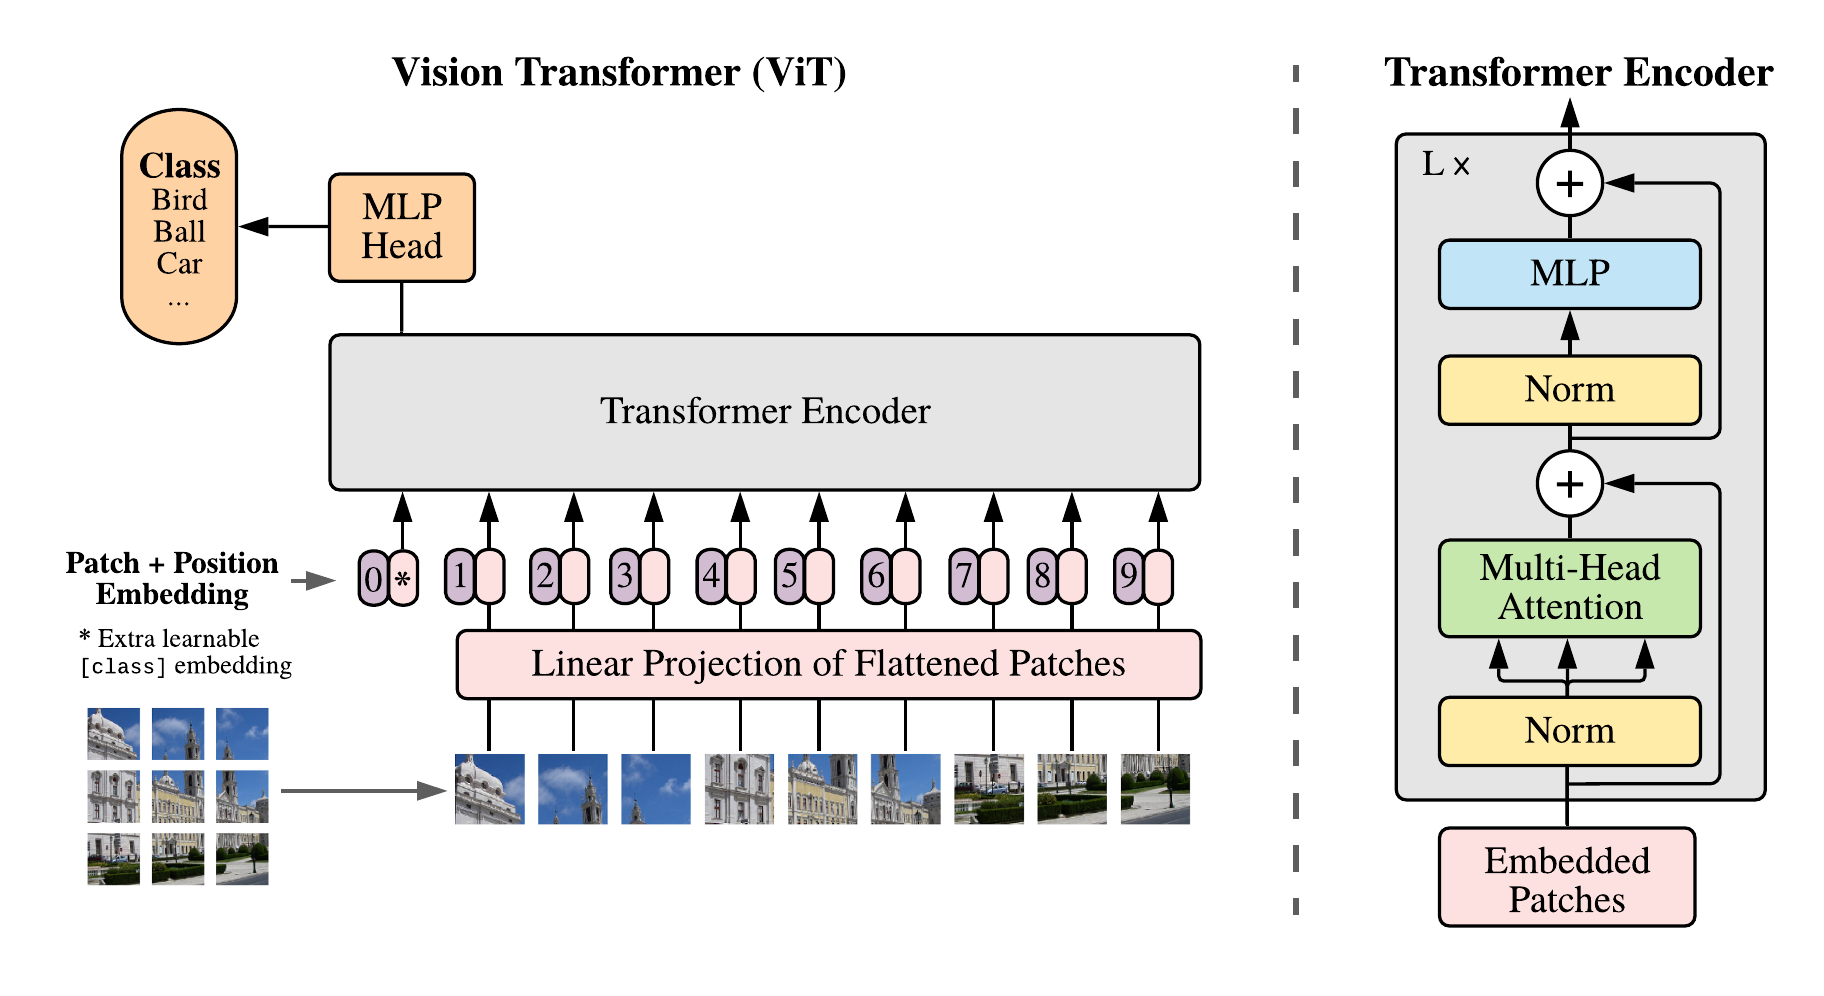
\includegraphics[width=1\textwidth]{vision-transformer-arch.png}
    \caption{Архітектура моделі}
    \label{fig:model-arch}
\end{figure}

\subsection{Vision Transformer}
Огляд моделі наведено на рисунку \ref{fig:model-arch}.
Стандартний трансформатор отримує на вхід 1D
послідовність ембедингів токенів.
Для обробки 2D-зображень ми змінюємо розмірність зображення
$x \in \mathbb{R}^{H\times W \times C}$ у послідовність
зплющених 2D регіонів $x_p \in \mathbb{R}^{N\times (P^2\cdot C)}$,
де $(H, W)$ -- роздільна здатність початкового
зображення, $C$ -- кількість каналів, $(P, P)$ -- роздільна
здатність кожного регіону зображення,
а $N = HW / P^2$ -- результуюча кількість регіонів,
яка також служить ефективною довжиною вхідної послідовності для
трансформера. Трансформер використовує
латентний векторний постійного розміру $D$ у всіх своїх шарах,
тому ми випрямляємо регіони та відображаємо у розмір $D$
за допомогою тренованої лінійної проекції (рівняння \ref{eq:1}).
Ми називаємо результат цієї проекції ембедінгами регіонів.

Так як ми працюємо не з послідовностями, ми додаємо
тренований ембедінг до послідовності ембедингів регіонів
$z_0^0 = x_{\text{class}}$. Його стан на виході енкодеру трансформера
($z_L^0$) служить як представлення зображення $y$ (рівняння \ref{eq:4}).
Як під час попереднього тренування, і під час точної настройки,
головка класифікації приєднана до  $z^0_L$.
Класифікаційна головка являє собою багатошаровий перцептрон
з одним прихованим
шаром під час попереднього тренування та одним лінійним шаром
під час точної настройки.

Ембединги позиції додаються до ембедингів регіонів,
щоб зберегти позиційну інформацію. Ми використовуємо стандартні
вбудовувані позиції одинарної розмірності, оскільки ми не
спостерігали значних прирістів продуктивності від використання
більш складних ембедингів, що усвідомлюють двухмірну природу
зображень. Отримана послідовність вбудованих векторів
служить вхідними даними для енкодера.

Енкодер трансформера складається з чергування шарів багатоголовкової
уваги, та блоків перцептрону (рівняння \ref{eq:2}, \ref{eq:3}).
Перед кожним блоком застосовується шарова нормалізація (LN),
та залишкові з'єднання після кожного блоку. Багатошаровий перцептрон
використовує нелінійність GELU \cite{gelu}.

\begin{align}
    z_0 &= [x_{{class}};x_p^1 E;x_p^2 E; ...; x_p^N E] +E_{pos} \label{eq:1}\\
    E &\in \mathbb{R}^{(P^2 \cdot C)\times D},
    E_{pos} \in \mathbb{R}^{(N+1)\times D} \nonumber\\
    z'_l &= {MSA}({LN}(z_{l-1})) + z_{l-1}, &l=1...L \label{eq:2}\\
    z_l &= {MLP}({LN(z'_l)})+z'_l, &l=1...L \label{eq:3}\\
    y &= {LN}(z_L^0) \label{eq:4}
\end{align}

\subsubsection{Індуктивне зміщення.}
Ми зазначаємо, що Vision Transformer (ViT) має набагато менше
специфічного для зображення індуктивного зміщення, ніж ЗНМ.
У ЗНМ локальність, двовимірна структура сусідства
та еквівалентність переміщення вписуються в кожен шар по всій моделі.
У ViT лише щільні шари є локальними та поступально еквіваріантними,
тоді як шари самоуваги є глобальними. Двовимірна структура сусідства
використовується дуже економно: на початку моделі шляхом
розрізання зображення на регіони та під час точного налаштування,
та для регулювання позиційних ембедингів для зображень з
різною роздільною здатністю.
Крім цього, позиційні ембединги під час ініціалізації
не містить інформації про 2D-позиції регіонів,
і всі просторові відносини між регіонами повинні вивчатися з нуля.

\subsubsection{Гібридна архітектура.}
Як альтернативу необробленим регіонам зображень,
вхідну послідовність можна сформувати за допомогою функцій ЗНМ.
У цій гібридній моделі проекція ембедінгу регіона $E$
(рівняння \ref{eq:1}) застосовується до регіонів,
витягнутих з представлення ЗНМ. Як особливий випадок, патчі можуть
мати просторовий розмір $1 \times 1$, що означає, що вхідна
послідовність отримується простим випрямленням просторових
розмірів представлення та проеціюванням на розмір трансформера.
Ембедінг класифікації вхідних даних та ембедінги
позицій додаються як описано вище.

\subsection{Точне налаштування та більша роздільна здатність}
Зазвичай ми попередньо тренуємо ViT на великих датасетах,
і точно налаштовуємо до меньших поточних завдань. Щоб це зробити,
ми видаляємо попередньо навчену головку прогнозування
та приєднуємо ініціалізований нулями шар прямого переходу
$D \times K$, де $K$ -- кількість класів у поточній задачі.
Часто вигідніше точно налаштувати на більшій роздільній здатності,
ніж попереднє тренування. Під час подавання зображень із більш високою
роздільною здатністю розмір регіона залишається однаковим,
що призводить до більшої ефективної довжини послідовності.
Vision Transformer може обробляти довільні довжини послідовностей
(до обмежень пам’яті), однак попередньо навчені позиційні
ембединги можуть втратити своє значення. Тому ми виконуємо
2D інтерполяцію попередньо навчених вкладених позицій відповідно
до їх розташування на вихідному зображенні. Зауважте, що це
регулювання роздільної здатності та вилучення регіонів -- це єдині
точки, при яких індуктивне зміщення щодо 2D-структури зображень
вручну вводиться в Vision Transformer.
